% ==========================================================================
% NeurIPS 2026 workshop build — DOUBLE-BLIND (anonymized by the class).
% Build: tectonic workshop.tex . Shares body.tex with arxiv.tex.
% ==========================================================================
\documentclass{article}
\usepackage[dblblindworkshop]{neurips_2026} % double-blind workshop; loads natbib; anonymizes authors

\usepackage[T1]{fontenc}
\usepackage{lmodern}
\usepackage{microtype}
\usepackage{hyperref}
\usepackage{url}
\usepackage{booktabs}
\usepackage{amsmath,amssymb}
\usepackage{graphicx}
\usepackage{xcolor}
\usepackage{pgfplots}
\pgfplotsset{compat=1.17}

\newcommand{\sys}{\textsc{MemMux}}
\newcommand{\code}[1]{\texttt{#1}}
% Anonymized build: do NOT reveal the repository (it deanonymizes the author).
\newcommand{\repourl}{\footnote{Code, benchmark, and a one-command reproducer are open-source and
will be released; the repository URL is withheld to preserve double-blind review.}}

\title{\sys{}: Runtime Verification and Honest Resource Attribution\\
for Fleets of Parallel Coding Agents}

% The workshop template requires both \title and \workshoptitle.
\workshoptitle{Who Verifies the Agents? NeurIPS 2026 Workshop}

\author{Anonymous Author(s)} % anonymized by the dblblindworkshop option

\begin{document}
\maketitle
% ==========================================================================
% Shared body for both builds (arxiv.tex = named preprint; workshop.tex =
% double-blind NeurIPS workshop). Wrappers define \sys, \code, \repourl,
% the title/author block, and load the packages.
% ==========================================================================

\begin{abstract}
Developers increasingly run not one coding agent but a fleet of them side by side on a single
workstation. The tools they reach for---terminal multiplexers like \code{tmux} and a new generation
of agent managers---were built to arrange windows, not to govern memory. When ten agents each spawn
language servers, test runners, and browsers, nothing on the machine can say how much memory belongs
to which agent, guarantee that a terminated agent's descendants are actually gone, notice a child
that has escaped its agent, or keep the machine off the swap cliff without an OOM kill silently
discarding uncommitted work. We argue these are \emph{verification} problems: an agent-hosting
substrate should continuously emit signals an operator (or an auditor) can check. We present \sys{},
a local runtime that treats resource governance as a set of checkable guarantees---honest per-agent
attribution, complete reclamation, escaped-process visibility, bounded footprint under overcommit,
and low monitoring overhead---and a claims-disciplined benchmark that measures each guarantee against
\code{tmux}, a purpose-built agent multiplexer, and a raw-process baseline running identical
workloads. On a 32\,GB Linux reference host, as the fleet grows to ten agents, \sys{} holds peak
footprint flat at 435\,MiB while the ungoverned tools grow linearly to 2.1\,GB; it reclaims 100\% of
a terminated agent's process subtree where the raw baseline strands half of it (ten orphaned
processes, 303\,MiB, at $N{=}10$); and it is the only system that surfaces an escaped child, detecting
10/10 injected escapes versus a capability the others structurally lack. We report an honest cost:
the always-on 1\,Hz attribution scan stays near 0.6\% CPU for a single agent but reaches 2.7\% at ten,
over our 2\% target. We release the engine, the benchmark, and a one-command reproducer.
\end{abstract}

\section{Introduction}

A year ago, running an autonomous coding agent meant babysitting a single session. Today it is
normal to fan a task out across several agents at once---one refactoring, one writing tests, one
chasing a flaky build---and to watch them in a grid of panes. The agents themselves have improved
quickly~\citep{yao2023react,shinn2023reflexion,jimenez2024swebench,yang2024sweagent}; the substrate
they run on has not. Developers arrange these fleets with terminal multiplexers such as
\code{tmux}~\citep{tmux} or with purpose-built agent managers, and both were designed to place
windows on a screen, not to answer questions about memory.

Those questions matter because a coding agent is not a single process. It is a tree: the model's
CLI, a shell, language servers, test and build workers, sometimes a headless browser. A handful of
such trees can exhaust a laptop's RAM. When they do, the operating system's response---the Linux OOM
killer, or swap thrashing---is blunt and invisible: a process is killed mid-write, or the whole
machine grinds, and the agent's uncommitted edits are simply gone. Nothing in the stack was
accountable for that memory in the first place. \code{tmux} does not know that pane 7's language
server belongs to the same logical agent as pane 3's test runner; it cannot tell you that a
double-forked child has escaped supervision; and it has no budget it is trying to keep.

We think the right lens for this is \emph{runtime verification}~\citep{bartocci2018introrv}: rather
than prove properties of the substrate ahead of time, instrument it so the properties it claims can
be \emph{checked while it runs}, and surface any violation rather than hide it. Cluster schedulers
made an analogous move a decade ago---Borg combined admission control, over-commitment, and
process-level isolation, and treated monitoring as a first-class output~\citep{verma2015borg}. We
bring that stance down to a single developer machine and to the specific failure modes of agent
fleets.

This paper contributes: (i) \textbf{five verification signals for agent fleets}
(Section~\ref{sec:signals})---honest per-agent attribution, complete reclamation on teardown,
escaped-process visibility, bounded footprint (and preserved work) under overcommit, and bounded
monitoring overhead---each a monitor with a stated threshold; (ii) \textbf{\sys{}}
(Section~\ref{sec:design}), a local runtime that enforces them; and (iii) \textbf{a claims-disciplined
benchmark} (Section~\ref{sec:method}) that drives \code{tmux}, an agent multiplexer, and a raw
baseline through \emph{identical} deterministic workloads, tags every process as agent or manager
overhead, and never reports a number it did not measure---where a competitor cannot be driven
honestly, it is recorded as skipped, not estimated. On a 32\,GB Linux reference host the guarantees
hold and, under overcommit, separate \sys{} from the ungoverned tools by $\sim$5$\times$ at ten
agents (Section~\ref{sec:eval}). We are candid about scope: the workload is a deterministic stub
rather than live models, the fleets are modest ($N \le 10$), and the monitoring cost is not yet
under 2\%---all discussed in Section~\ref{sec:limits}.

\section{Background and Related Work}

\paragraph{Language-model agents.} Interleaving reasoning with tool use~\citep{yao2023react} and
adding self-reflection~\citep{shinn2023reflexion} turned language models into agents that take long
sequences of actions. Coding is the canonical proving ground: SWE-bench frames the task as resolving
real GitHub issues against a repository~\citep{jimenez2024swebench}, and SWE-agent shows a
well-designed agent--computer interface matters as much as the model~\citep{yang2024sweagent}.
Multi-agent settings, first studied for open-ended behavior~\citep{park2023generative}, are now a
practical reality on developer machines. This work is orthogonal to the agents: we govern whatever
they spawn.

\paragraph{Terminal multiplexers.} \code{tmux}~\citep{tmux} is the default way developers run many
long-lived sessions at once. It is excellent at persistent panes and detach/reattach---the honest
baseline any ``run many agents'' tool must beat---but a pane is just a process group under a server
with no notion of a logical agent, a memory budget, or a process that has wandered out of its
subtree.

\paragraph{Resource management.} Cluster managers solved fleet-scale governance long ago: Borg with
admission control and over-commitment~\citep{verma2015borg}, Mesos with two-level
scheduling~\citep{hindman2011mesos}, and Kubernetes as the open-source lineage~\citep{kubernetes}.
The enforcement primitives they use---Linux control groups~\citep{cgroupv2} and the OOM
killer~\citep{linuxoom}---live in every modern kernel. \sys{} borrows the ideas (reserve, admit,
reclaim before you thrash) but targets a single un-orchestrated laptop, and it deliberately avoids
hard cgroup containment in favor of signal-based supervision so it runs unprivileged.

\paragraph{Memory accounting.} Summing resident set size (RSS) over a process tree double-counts
shared pages. The proportional set size (PSS) exposed through \code{/proc/<pid>/smaps\_rollup}
divides each shared page by its sharers and is the honest per-process figure~\citep{procfs}; macOS
offers \code{phys\_footprint} as its analogue. \sys{} attributes by PSS (RSS fallback) so a task's
number reflects memory it is responsible for.

\paragraph{Runtime verification.} Rather than verify a system statically, runtime verification
instruments it and checks a specification against the execution trace, reacting to
violations~\citep{bartocci2018introrv}. Our five signals are exactly such monitors: cheap, always-on
checks with explicit thresholds whose failures are events, not silence.

\section{The Design of \sys{}}
\label{sec:design}

\sys{} is a Rust workspace: a daemon (\code{memmuxd}) that owns state and does the governing, and a
terminal client that attaches over a Unix domain socket. A \emph{task} is a durable, logical agent;
a \emph{runtime} is one physical launch of a provider inside a pseudo-terminal. The design is
organized around making each signal checkable.

\paragraph{Attribution.} Once per second the daemon snapshots the host process tree and, for each
running task's provider root, sums the PSS of the root and all descendants. That per-task figure
feeds the budget, the client's task view, and---because we record which pids were seen under each
root---the escaped-process check. Attribution is scoped to processes \sys{} launched, so unrelated
host activity never pollutes a task's number.

\paragraph{Recursive reclamation.} When a task is terminated (by the operator or because its provider
exited), \sys{} reaps the \emph{entire} owned subtree. The order is load-bearing: the subtree is
signalled while the root is alive, because once the root dies its children reparent to \code{init}
and the tree that identifies them is lost. For a provider that already exited, \sys{} reaps from the
pids recorded while the task ran. The target is $\geq 99.5\%$ of owned descendants gone within ten
seconds.

\paragraph{Escaped-process reconciliation.} A child that double-forks and reparents to \code{init}
has escaped its agent---the classic way a leak hides. Each sample, \sys{} reconciles the pids seen
under a task against the live tree; a once-owned pid now living outside every task subtree is flagged
\emph{escaped} and surfaced as an event. Reconciliation is scoped to the managed set, so the signal
is a real ``we lost track of a process we started,'' not host noise.

\paragraph{Admission and the pressure ladder.} The daemon holds a memory budget (physical RAM minus
reserves for the OS, interactive apps, and a swap-safety margin). Starting a task reserves its
predicted peak; if the reservation would exceed the budget the task stays queued with a visible
reason rather than over-subscribing the machine. When live usage climbs anyway, a graduated
\emph{pressure ladder} responds before the machine thrashes: reclaim escaped children, hibernate the
lowest-priority idle task, recycle the largest provider, and---only at the top, and only after
persisting a checkpoint of the victim's Git state---terminate the lowest-priority tree. Preserving
work always precedes destroying a process. Every governance action writes an audit decision with its
reason and evidence, which is what makes the system verifiable rather than merely automatic.

\section{Verification Signals and Methodology}
\label{sec:signals}
\label{sec:method}

We frame governance as five monitors, each with a threshold (Table~\ref{tab:signals}). A benchmark
harness drives every system under test through identical, deterministic workloads and evaluates the
monitors from an external process sampler---the same accounting code the daemon uses, pointed at
whatever root pids a launcher reports, so measurement is product-agnostic.

\begin{table}[t]
\centering\small
\begin{tabular}{@{}llp{7.2cm}@{}}
\toprule
& \textbf{Signal} & \textbf{Monitor / threshold} \\
\midrule
H1 & Attribution        & $\geq 95\%$ of a launched tree's proportional memory mapped to its owning task \\
H2 & Cleanup            & $\geq 99.5\%$ of an owned subtree gone $\leq 10$\,s after the launcher's normal teardown \\
H3 & Escaped visibility & every process that escapes its agent is surfaced as an event \\
H4 & Bounded / no-loss  & footprint held near budget under overcommit; uncommitted work checkpointed before any reclaim \\
H5 & Overhead           & continuous monitoring costs $\leq 2\%$ CPU at fleet scale \\
\bottomrule
\end{tabular}
\caption{The five runtime-verification signals and their pass thresholds.}
\label{tab:signals}
\end{table}

\paragraph{Launchers.} Each launcher starts $N$ identical agents and reports the pids that constitute
the fleet: a \emph{raw} baseline (spawn the stub directly), \code{tmux} (one pane per agent on an
isolated server), and \sys{} (create $N$ tasks through the real daemon). A fourth, the \code{herdr}
agent multiplexer, is driven through its socket API where installed; on our stock Linux reference host
it was absent and is reported as skipped rather than guessed, as are \code{dmux} (which requires a
controlling terminal and cannot be driven headlessly), \code{cmux}, and \code{agentmux}.

\paragraph{Workload.} A deterministic stub agent replays a recording of allocate / spawn-child / emit
/ sleep steps, touching every page it allocates so its resident memory is real. Using a stub rather
than a live model is a deliberate choice: it makes runs reproducible and identical across launchers,
at the cost of realism (Section~\ref{sec:limits}). A \emph{hold} scenario keeps $N$ agents, each with
a live child, concurrently resident for the measurement window; without it, short workloads finish
before a fleet can be observed---an error we hit and corrected early.

\paragraph{Claims discipline.} The harness records each launcher's version, the measurement date, and
the host; it tags every sampled process as agent or manager overhead so the two are reported
separately; and it emits a number only for a monitor it actually measured. A launcher that cannot be
driven contributes ``unsupported,'' never a fabricated zero. These rules are as much a contribution
as the engine: fair comparison of agent-hosting tools has no accepted methodology, and an unfair one
is worse than none.

\section{Evaluation}
\label{sec:eval}

\paragraph{Setup.} The reference host is an AWS \code{m7i.2xlarge}: 8 vCPUs (Intel Xeon Platinum
8488C), $\approx$31\,GiB RAM, an 8\,GiB swap file, Ubuntu 24.04 (Linux 6.17). Versions: \code{tmux}
3.4, \sys{} 0.8.0. Each cell is two trials; we report mean\,$\pm$\,95\% CI. We swept fleet sizes
$N \in \{1,5,10\}$ across three scenarios. A macOS cross-check (Apple M4 Max, 32\,GiB), which
additionally exercised \code{herdr}, agreed qualitatively: \code{herdr}, like the other ungoverned
managers, reaped its subtrees on teardown (100\% cleanup) but detected no escapes and grew its
footprint with the fleet.

\subsection{H4: bounded footprint under overcommit}

We give \sys{} a budget of 3000\,MiB---below the aggregate reservation of the larger fleets---and
start all $N$ agents under each launcher. Figure~\ref{fig:vsn} plots peak total footprint against
fleet size. The ungoverned launchers scale linearly: at ten agents they reach 2.1\,GB. \sys{} admits
what fits (one agent at $N{=}1$; two at $N{=}5$ and $N{=}10$, deferring the rest with a visible
reason---3 and 8 deferrals respectively) and holds peak footprint flat at 435\,MiB, a $4.9\times$
separation at $N{=}10$. This is the sharpest result in the paper and the one that most directly
motivates governance: without a budget, a fleet's footprint is simply the sum of its agents.

\begin{figure}[t]
\centering
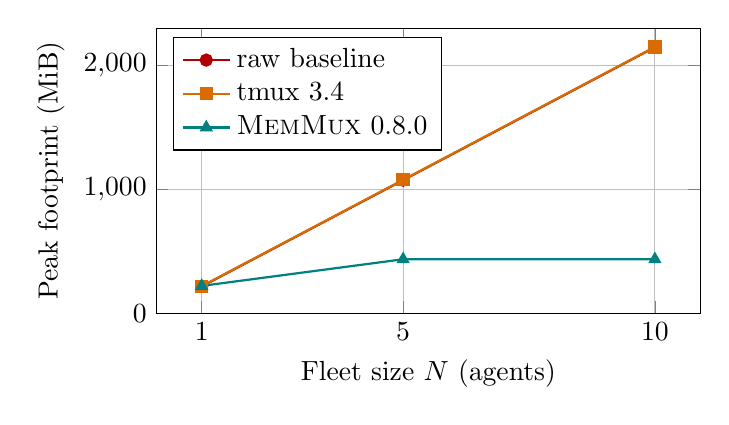
\begin{tikzpicture}
\begin{axis}[
  width=0.7\linewidth, height=5.2cm,
  xlabel={Fleet size $N$ (agents)}, ylabel={Peak footprint (MiB)},
  xtick={1,5,10}, ymin=0, ymax=2300,
  legend pos=north west, legend cell align=left, grid=major,
  mark size=2pt,
]
\addplot[thick,red!70!black,mark=*]     coordinates {(1,215.3)(5,1073.7)(10,2146.2)}; \addlegendentry{raw baseline}
\addplot[thick,orange!85!black,mark=square*] coordinates {(1,217.7)(5,1076.1)(10,2148.6)}; \addlegendentry{tmux 3.4}
\addplot[thick,teal,mark=triangle*]     coordinates {(1,219.9)(5,434.8)(10,434.8)}; \addlegendentry{\sys{} 0.8.0}
\end{axis}
\end{tikzpicture}
\caption{Peak fleet footprint under a 3000\,MiB budget (\emph{overcommit}). Ungoverned tools scale
linearly with the fleet; \sys{} stays flat by deferring admissions ($4.9\times$ lower at $N{=}10$).}
\label{fig:vsn}
\end{figure}

The \emph{no-lost-work} half of H4 is a capability we verify but did not trigger here: because \sys{}
defers at admission, the pressure ladder rarely needs to reclaim a running victim. A daemon-level test
confirms the guarantee directly---a task with a dirty Git worktree, forced into the emergency stage,
produces a checkpoint carrying its patch hash \emph{before} the process is terminated. Ungoverned
launchers have no checkpoint mechanism, so this is reported as a capability they lack, not a number.

\subsection{H2: complete cleanup on teardown}

Each launcher starts a fleet whose agents each hold a memory-bearing child, then is torn down exactly
as it normally would be (raw: kill the roots; \code{tmux}: \code{kill-server}; \sys{}: terminate each
task). Ten seconds later we count survivors from the owned set (Table~\ref{tab:h2}). The raw baseline
strands every child it spawned---its teardown kills only the roots, orphaning the grandchildren---and
the leak grows with the fleet, to ten processes and 303\,MiB at $N{=}10$. \code{tmux} and \sys{} both
reap their full subtree at every size.

\begin{table}[t]
\centering\small
\begin{tabular}{@{}lrrrr@{}}
\toprule
Launcher & Fleet $N$ & Leaked procs & Leaked MiB & Reclaimed \\
\midrule
raw-baseline & 1  & 1  & 30.6  & 50.0\% \\
raw-baseline & 5  & 5  & 151.8 & 50.0\% \\
raw-baseline & 10 & 10 & 303.0 & 50.0\% \\
tmux 3.4     & 10 & 0  & 0.0   & 100.0\% \\
\sys{} 0.8.0 & 10 & 0  & 0.0   & 100.0\% \\
\bottomrule
\end{tabular}
\caption{Survivors after normal teardown (\emph{hold}). The raw baseline leaks half of every fleet;
\code{tmux} and \sys{} reclaim 100\% at all $N$.}
\label{tab:h2}
\end{table}

The honest reading: on \emph{explicit} teardown, cleanup separates \sys{} from the raw baseline, not
from a real multiplexer---\code{tmux} reaps its subtrees too. This is the kind of result the claims
discipline exists to surface.

\subsection{H3: escaped-process visibility}

We inject escapes: a stub forks an intermediate that spawns a memory-holding grandchild and then
exits, reparenting the grandchild to \code{init} while it stays alive. The harness independently
confirms the reparenting, then asks each launcher what it detected (Table~\ref{tab:h3}). \sys{}
surfaces every escape---1/1, 5/5, 10/10---through events read from the daemon; the baselines have no
mechanism to notice. This is a capability, not a tuning difference, and it is the cleanest
separation from a real competitor.

\begin{table}[t]
\centering\small
\begin{tabular}{@{}lrrl@{}}
\toprule
Launcher & Injected & Detected & Note \\
\midrule
raw-baseline & 10 & --- & unsupported \\
tmux 3.4     & 10 & --- & unsupported \\
\sys{} 0.8.0 & 1 / 5 / 10 & 1 / 5 / 10 & detected all, every $N$ \\
\bottomrule
\end{tabular}
\caption{Escaped-process detection (\emph{escape}). ``---'' denotes no detection mechanism; it is
never scored as zero-of-measured.}
\label{tab:h3}
\end{table}

\subsection{H1 and H5: attribution and the cost of governance}

Across every run \sys{} attributed 100\% of each launched tree's proportional memory to its owning
task (H1). The cost of governance in \emph{memory} is small and we report it plainly: the \sys{}
daemon's own resident footprint is 4.6--5.4\,MiB (growing slightly with the fleet), against 2.4\,MiB
for the \code{tmux} server and zero for the raw baseline. The cost in \emph{CPU} is the honest weak
spot (H5): the always-on 1\,Hz full-tree PSS scan costs 0.6\% CPU at a single agent, 1.5\% at five,
and 2.7\% at ten---over our 2\% target once the fleet reaches ten. The scan is $O(\text{processes})$
and currently re-reads the whole tree each tick; incremental sampling that touches only changed pids
is the obvious fix and is future work. We state the miss rather than bury it.

\section{Discussion and Limitations}
\label{sec:limits}

\paragraph{Synthetic workload.} The largest threat to validity: agents are a deterministic
memory-ballast stub, not live models. We trade realism for reproducibility and for identical
workloads across launchers, which is what makes the comparison fair. The \emph{qualitative}
guarantees---attribution, cleanup, escape visibility, admission---do not depend on the workload, but
the specific megabytes for a real Claude- or GPT-driven session will differ, and validating on live
agents is the most important next step.

\paragraph{One host, modest fleets.} We evaluate a single 32\,GB Linux host (with a macOS cross-check)
and $N \le 10$. The harness sweeps to $N{=}20$ and the reproducer emits the full curve; we simply did
not run larger fleets, on which the CPU-overhead question (H5) becomes sharper.

\paragraph{Conservative admission.} \sys{} reserves each task's class-predicted peak, which for our
stub is well above its actual RSS---so the flat 435\,MiB in Figure~\ref{fig:vsn} reflects admission
protecting against the \emph{reservation}, and \sys{} leaves headroom on the table (it deferred agents
that would have fit). An exponentially-weighted predictor that tightens reservations toward observed
peaks is designed and is future work. The bounded-footprint claim stands; the specific admit count
would rise with a tighter predictor.

\paragraph{Overhead not yet met; empirical, not formal.} Monitoring exceeds 2\% CPU by ten agents
(above), and these are runtime monitors with measured pass/fail behavior, not machine-checked proofs.
We claim the signals are checkable and checked, not that the engine is formally verified.

\section{Reproducibility}
\label{sec:repro}

\sys{} and its benchmark are open source (MIT).\repourl{} A single command runs the full matrix---every
launcher, scenario, and fleet size, with repeated trials---captures the host specification, and
regenerates every table and figure here plus the raw per-sample and per-process time series.
Competitor versions and the measurement date are embedded in the generated report, and any launcher
that could not be driven is listed with its reason. Reproducing the evaluation on another host is one
invocation.

\section{Conclusion}

Fleets of coding agents have outrun the tools we use to run them: multiplexers arrange them, but
nothing governs them. We argued that memory governance for such fleets is a verification problem and
built \sys{} to make five guarantees checkable at runtime, with a benchmark honest enough to admit
where those guarantees do \emph{not} distinguish us. On a 32\,GB Linux host the payoff is concrete---a
flat versus linear footprint under overcommit ($4.9\times$ at ten agents), complete cleanup where the
raw baseline strands half a fleet, and full visibility into escaped processes that the alternatives
cannot see---alongside an honest overhead cost we have not yet driven under 2\%. The path from here is
a live-agent workload and larger fleets; the reproducer makes both a single command away.

\small
\bibliographystyle{plainnat}
\bibliography{refs}

\normalsize
\appendix
\section{Reproducer invocation}
The canonical run and a fast smoke run:
\begin{verbatim}
memmux-bench paper --out paper-out
memmux-bench paper --agents-sweep 1,5,10 --scenarios hold,escape,overcommit \
    --trials 2 --agent-budget-mib 3000 --out linux-run
\end{verbatim}
Each writes \code{host.json}, a Markdown report, per-cell \code{*.jsonl} and \code{*.procs.jsonl}
time series (RSS, PSS, USS, swap, and page faults per process on Linux), and the figures. The report
header records OS, architecture, physical RAM, CPU model, core count, and tool versions.

\end{document}
